%Dernière modification JG: 11 novembre 2020
\RequirePackage[l2tabu, orthodox]{nag} %Check for obsolete commands
\documentclass[canadien,12pt,oneside,letterpaper]{article}
%
%-----------------------------------------------------
%Loading packages
%
\usepackage[utf8]{inputenc}
\usepackage[T1]{fontenc}
\usepackage[canadien]{babel}
\usepackage{lmodern}
\usepackage{textcomp}
\usepackage{amsmath,amssymb}
\usepackage{siunitx}
\usepackage{xcolor}
\usepackage{hyperref}
\usepackage[all]{hypcap}
\usepackage{graphicx}
\usepackage[americanvoltages,americancurrents,siunitx]{circuitikz}
\usetikzlibrary{babel}
\usepackage{caption}
\usepackage[letterpaper,headheight=15pt]{geometry}
\usepackage{fancyhdr}
\usepackage{setspace}
%
%----------------------------------------------------
%Other configurations and layout
%
\sisetup{separate-uncertainty}
\captionsetup{font=small,labelfont=bf,margin=0.1\textwidth}
\pagestyle{fancy}
\fancyhf{}
\lhead{\textsl{GPH-2006/PHY-2002~---~Laboratoire~VIII}}
\rhead{\textsl{Page \thepage}}
\setcounter{secnumdepth}{0}
\setlength{\parskip}{1.5ex plus0.5ex minus0.2ex}
\setlength\parindent{0pt}
%\onehalfspacing
\interfootnotelinepenalty=10000 %To avoid footnotes spreading on several pages.
%
%---------------------------------------------------
%
\title{\textbf{Complément}\\Oscillateurs électroniques\thanks{Auteurs: Claudine Allen, Jérémie Guilbert \& Jean-Raphaël Carrier}}
\renewcommand\footnotemark{}
\date{}

\begin{document}
\maketitle \vspace{-2cm}

% À l’inverse de filtrer des fréquences d’un signal, cet atelier explore comment ajouter de nouvelles fréquences. La génération de ces signaux oscillant périodiquement à partir d’un courant constant fera notamment intervenir la fonction de comparateur de l’amplificateur opérationnel pour contrôler le cycle de charge-décharge d’un condensateur, puis celle d’amplification avec rétroaction où la fréquence d’oscillation est sélectionnée avec un filtre passe-bande. L’étudiant.e sera aussi initié.e à la conception d’un circuit LC résonnant à une fréquence d’oscillation requise. Des fonctions d’intérêt pour les circuits oscillateurs étudiés sont d’actionner un transducteur afin d’obtenir des ondes mécaniques, ou encore de définir un étalon de temps lorsque l’oscillation est pratiquement harmonique avec une seule fréquence. %La transduction sera d’abord mise en pratique avec un haut-parleur pour générer des ondes sonores, et puis avec la résonance de vibration d’un cristal de quartz pour obtenir une oscillation quasi-monochrome qui définira la seconde.

Bien que les filtre puissent être utilisés passivement pour simplement atténuer les signaux qui oscillent à certaines fréquences, il est aussi possible de les utiliser en combinaison avec des amplificateurs opérationnels afin de générer activement des signaux à des fréquences voulues. La génération de ces signaux fait intervenir la fonction de comparateur d'un ampli-op afin de contrôler le cycle de charge-décharge d'un condensateur, puis celle d'amplification avec rétroaction afin de sélectionner la fréquence d'oscillation avec un filtre passe-bande. Des fonctions d’intérêt pour les circuits oscillateurs étudiés sont d’actionner un transducteur afin d’obtenir des ondes mécaniques, ou encore de définir un étalon de temps lorsque l’oscillation est pratiquement harmonique avec une seule fréquence.

\section{Oscillateur à relaxation avec comparateur}
\begin{figure}[h]
\centering
\begin{circuitikz} \draw
(0,0) node[op amp](opamp){}
(opamp.+) to[short] (-1.2,-0.5) to[short] (-1.2,-2.2)
(opamp.-) to[short] (-1.2,0.5) to[short] (-1.2,2.2)
(opamp.out) to[short,-o] (2.1,0) node[right]{$v_{\mathrm{out}}$}
(opamp.down) ++ (0,-0.5) node[below]{$-5$~V} -- (opamp.down)
(opamp.up) ++ (0,0.5) node[above]{5~V} -- (opamp.up)
(-4,2.2) node[ground]{} to[C=$C$] (-1.2,2.2) to[R=$R$] (1.6,2.2) to[short] (1.6,-2.2) to[R=10~k$\Omega$] (-1.2,-2.2) to[R=10~k$\Omega$] (-4,-2.2) node[ground]{}
;\end{circuitikz}
\caption{\label{sch-osc-relax}Oscillateur à relaxation avec comparateur}
\end{figure}
%Ancienne légende de la figure 1
Ce circuit, illustré à la figure \ref{sch-osc-relax}, est basé sur l'utilisation de la fonction comparateur de l'ampli-op qui permet de contrôler le cycle de charge-décharge d'un condensateur afin de générer des oscillations à une fréquence déterminée par les valeurs des composants du circuit. Le condensateur qui se charge cause éventuellement l'entrée inverseuse de l'amplificateur opérationnel à dépasser celle non inverseuse et la tension de sortie de ce comparateur tombe alors négative, renversant ainsi la polarité appliquée sur le condensateur. Celui-ci se décharge maintenant jusqu'à ce que l'entrée inverseuse repasse sous celle non inverseuse et remet la sortie positive pour recommencer le cycle. 

\section{Oscillateur harmonique à rétroaction - pont de Wien}
\begin{figure}[h]
\centering
\begin{circuitikz} \draw
(0,0) node[op amp](opamp){}
(opamp.+) to[short] (-1.2,-0.5) to[short] (-1.2,-2.2)
(opamp.-) to[short] (-1.2,0.5) to[short] (-1.2,2.2)
(opamp.out) to[short,-o] (2.1,0) node[right]{$v_{\mathrm{out}}$}
(opamp.down) ++ (0,-0.5) node[below]{$-5$~V} -- (opamp.down)
(opamp.up) ++ (0,0.5) node[above]{5~V} -- (opamp.up)
(-4,2.2) node[ground]{} to[R=1~k$\Omega$] (-1.2,2.2) to[R=10~k$\Omega$] (1.6,2.2) to[short] (1.6,0) to[C=$C$] (1.6,-2.2) to[R=$R$] (-1.2,-2.2)
(-1.2,-2.2) to[C=$C$] (-3,-2.2) node[ground]{} to[R=$R$] (-3,-0.5) to[short] (-1.2,-0.5)
;\end{circuitikz}
\caption{\label{sch-osc-Wien}Oscillateur harmonique à rétroaction - pont de Wien}
\end{figure}
Ce circuit, illustré à la figure \ref{sch-osc-Wien}, utilise l'ampli-op en mode rétroaction afin de sélectionner la fréquence du signal qui entrera à l'entrée non inverseuse au moyen d'un filtre passe-bande, permettant par le fait-même de contrôler la fréquence des oscillations à la sortie.

Le signal à l'entrée non inverseuse, qui n'est \textit{a priori} que du bruit car aucune source n'est présente, est amplifié puis passe au travers d'un pont de Wien qui le filtre. Le signal ainsi filtré retourne ensuite à l'entrée de l'amplificateur pour être à nouveau amplifié et filtré, et ainsi de suite, \textit{ad infinitum}. Le pont de Wien est \textit{grosso modo} l'addition d'un filtre passe-bas et d'un filtre passe-haut pour former un filtre passe-bande. La fréquence du signal de sortie est $f=\left(2\,\pi\,R\,C\right)^{-1}$. L'amplitude finale du signal est fixée par la source d'alimentation de l'ampli-op. % Cet oscillateur doit son oscillation au chargement/déchargement du condensateur qui relie l'entrée non inverseuse de l'amplificateur au \textit{ground}.

\section{Oscillateur harmonique à rétroaction (LC)}
%Ancienne intro partie 3
Un autre oscillateur reposant sur le même principe de filtrage et amplification en boucle du signal est l'oscillateur LC. Vous avez étudié au dernier atelier le filtre RLC passe-bande dont le gain et la fréquence de résonance peuvent être déterminés analytiquement à partir des valeurs de résistance $R$, d'inductance $L$ et de capacitance $C$ du circuit. On pourrait donc remplacer le pont de Wien du dernier oscillateur par un circuit RLC afin d'obtenir, avec un choix judicieux des composants du circuit, une fréquence de résonance et un gain quelconques. 
\subsection{Fréquence de résonance et équation différentielle d'un oscillateur}
On peut déterminer la fréquence de résonance d'un circuit oscillateur en déterminant l'équation différentielle décrivant la tension ou le courant au point du circuit qui nous intéresse. Pour ce faire, les étapes générales sont les suivantes:
\begin{enumerate}
    \item Déterminer l'équation gouvernant le circuit à partir des lois de Kirchhoff.
    \item Substituer les équations consitutives tension/courant pour chacun des composants du circuit:
    \begin{itemize}
        \item Résistance : $V_R(t) = RI(t)$
        \item Condensateur : $I_C(t) = C\frac{dV(t)}{dt}$ ou $V_C(t) = V(0)+\frac{1}{C}\int_0^tI(t')dt'$
        \item Bobine : $V_L(t) = L\frac{dI(t)}{dt}$ ou $I_L(t) = I(0)+\frac{1}{L}\int_0^tV(t')dt'$
    \end{itemize}
    \item Exprimer l'équation différentielle en termes de la variable d'intérêt ($I$ ou $V$) au point désiré et résoudre l'équation.
\end{enumerate}

\begin{figure}[h]
\centering
\begin{circuitikz} \draw
(0,0) to[V=$V_S$,invert] (0,3) to[C=$C$] (3,3) to[R=$R$,i>^=$I$] (3,0) to[L=$L$] (0,0);
\end{circuitikz}
\caption{\label{circuitRLC-serie}Circuit RLC en série.}
\end{figure}

\vspace{0.7cm} Par exemple, pour le circuit RLC en série de la figure \ref{circuitRLC-serie}, on aurait, si on s'intéresse à déterminer l'expression pour le courant $I$, 
\begin{enumerate}
    \item $V_S(t)=V_C(t)+V_R(t)+V_L(t)$
    \item $V_S(t)=V(0)+\frac{1}{C}\int_0^tI(t')dt'+RI(t)+L\frac{dI(t)}{dt}$
\end{enumerate}
Si on suppose maintenant que la source produit une tension constante, on a, en prenant la dérivée de l'équation précédente, 
\begin{enumerate}
  \setcounter{enumi}{2}
  \item $\frac{dV_S(t)}{dt}=0=L\frac{d^2I(t)}{dt^2}+R\frac{dI(t)}{dt}+\frac{1}{C}I(t)$.
\end{enumerate}
Si on exprime l'équation de façon à ce que le coefficient du terme en dérivée seconde soit 1, on a 
\begin{equation}\label{eq:RCL}
    \frac{d^2I(t)}{dt^2}+\frac{R}{L}\frac{dI(t)}{dt}+\frac{1}{LC}I(t) = 0,
\end{equation}
qui est un équation différentielle ordinaire d'ordre 2 \textit{homogène}. Pour mieux visualiser la signification de chacun des termes de cette équation, il est utile d'utiliser une analogie avec un système plus intuitif, le système masse-ressort (figure \ref{systeme_masse_ressort}). À partir des forces identifiées sur la figure, l'équation du mouvement pour un objet de masse $m$ au bout d'un ressort de constante $k$ dans un milieu visqueux est 
\begin{figure}[h]
    \centering
    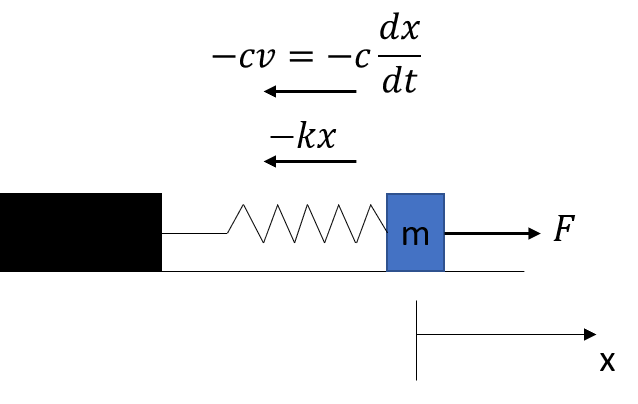
\includegraphics[]{Labos-Complements/Lab08/masse_ressort.png}
    \caption{\label{systeme_masse_ressort}Système masse-ressort sur une surface sans friction dans un milieu visqueux. Trois forces agissent sur la masse au bout du ressort: la force de rappel dictée par la constante de rappel du ressort $k$, une force de frottement fluide proportionnelle à la vitesse de la masse et au coefficient d'amortissement $c$ ainsi qu'une force extérieure $F$.}
    \label{fig:OF}
\end{figure}
\begin{equation}\label{eq:masse_ressort}
    \begin{split}
      &\sum F = m\frac{d^2x}{dt^2} = -c\frac{dx}{dt}-kx+F \\
      &\Rightarrow \frac{d^2x}{dt^2}+\frac{c}{m}\frac{dx}{dt}+\frac{k}{m}x = F.
    \end{split}
\end{equation}
S'il n'y a pas de force $F$ qui entretient le mouvement, l'équation \ref{eq:masse_ressort} a la même forme que l'équation pour le courant du circuit RLC avec une source constante. Cette équation, exprimée sous la forme canonique
\begin{equation}\label{eq:canonique}
    \frac{d^2I(t)}{dt^2}+2\alpha\frac{dI(t)}{dt}+\omega_0^2I(t) = 0,
\end{equation}
possède la solution générale
\begin{equation}\label{eq:sol_gen}
   I = Ae^{-\alpha t}\sin\left(\sqrt{\omega_0^2-\alpha^2}t+\phi\right), 
\end{equation}
où $A$ et $\phi$ sont des constantes déterminées par les conditions initiales du système, dans le cas où $\frac{\alpha}{\omega_0}<1$. Cette équation représente l'oscillation de la variable $I$ à la fréquence $\sqrt{\omega_0^2-\alpha^2}$. L'amplitude de l'oscillation, initialement de $A$, décroît de façon exponentielle avec le temps à un taux dicté par $\alpha$. En comparant terme à terme les équations \ref{eq:RCL}, \ref{eq:masse_ressort} et \ref{eq:canonique} avec cette solution, on observe une équivalence entre les termes résumée au tableau \ref{table-equiv_masse_ressort}.  

\begin{table}[h]
\centering
\begin{tabular}{c|ccc}
\hline
Interprétation physique & Amortissement & Oscillation & Terme d'entretien \\
Terme associé & $\frac{dI(t)}{dt}$ & $I(t)$ & \\
\hline
\textbf{Équation canonique} & $2\alpha$ & $\omega_0$ & ---\\
\textbf{Équation masse-ressort} & $\frac{c}{m}$ & $\sqrt{\frac{k}{m}}$ & $F$ \\
\textbf{Équation circuit RLC} & $\frac{R}{L}$ & $\frac{1}{\sqrt{LC}}$ & $\frac{dV_S}{dt}$ \\
\hline
\end{tabular}
\caption{\label{table-equiv_masse_ressort}Équivalences entre les termes de l'équation différentielle du système masse-ressort et celle du circuit RLC.}
\end{table}
Le tableau montre qu'on peut associer la résistance $R$ du circuit RLC au coefficient d'amortissement fluide $c$, celui-ci générant une force de frottement qui s'oppose au mouvement de la masse de façon proportionnelle à sa vitesse, semblable à la résistance qui crée une opposition au courant proportionnelle à sa dérivée temporelle. De même, les paramètres $L$ et $C$ peuvent être associés à la masse $m$ et à l'inverse de la constante de rappel du ressort $k$ respectivement. En l'absence de résistance, le système sera donc non-amorti et oscillera à la fréquence $\omega_0=\frac{1}{\sqrt{LC}}$. Si la résistance est non-nulle, la fréquence d'oscillation sera amortie et sera plutôt de $\sqrt{w_0^2-\alpha^2}=\sqrt{\frac{1}{LC}-\left(\frac{R}{L}\right)^2}$.  

La résolution de l'équation homogène décrite ici permet de trouver la fréquence de résonance d'un circuit. Pour déterminer la réponse en fréquence, c'est-à-dire la valeur du gain en fonction de la fréquence d'oscillation du signal d'entrée $V_S(t)$, il faut résoudre l'équation non-homogène. Ceci est habituellement réalisé en calculant la fonction de transfert du système directement dans l'espace des fréquences avec les expressions pour l'impédance des composants, tel que détaillé dans le complément \textit{Analyse fréquentielle}.

Noter qu'à partir de la solution dérivée pour le courant circulant dans le circuit RLC en série, on pourrait obtenir obtenir des équations pour la tension aux bornes de chacun des composants à partir des relations tension/courant. Par exemple, si on désire connecter une charge sur la bobine, on pourrait déterminer la tension à l'entrée de la charge en connaissant $I(t)$ et sachant que $V_L(t) = L\frac{dI(t)}{dt}$.

\section{Oscillations avec la puce 555}
%Ancienne sous-section
\begin{figure}[h]
\centering
\begin{circuitikz} \draw[thick]
(0,0) to[short] (0,0.5) node[right]{4} to[short,*-*] (0,1.5) node[right]{3} to[short] (0,2.5) node[right]{2} to[short,*-*] (0,3.5) node[right]{1} to[short] (0,4) to[short] (3,4) to[short] (3,3.5) node[left]{8} to[short,*-*] (3,2.5) node[left]{7} to[short] (3,1.5) node[left]{6} to[short,*-*] (3,0.5) node[left]{5} to[short] (3,0) to[short] (0,0)
{[anchor=east] (0,3.5) node{\textbf{GND}} (0,2.5) node{\textbf{TRIG}} (0,1.5) node{\textbf{OUT}} (0,0.5) node{\textbf{RESET}}}
{[anchor=west] (3,3.5) node{\textbf{V$_{\text{CC}}$}} (3,2.5) node{\textbf{DISCH}} (3,1.5) node{\textbf{THRES}} (3,0.5) node{\textbf{CONT}}}
;\end{circuitikz}
\caption{\label{sch-555}Schéma d'une puce 555.}
\end{figure}
La puce 555 est un circuit intégré (figure \ref{sch-555}) qui est très souvent utilisé en électronique pour, entre autres, bâtir un oscillateur.Les niveaux de déclenchement (\textit{trigger}) et de seuil (\textit{threshold}) valent un tiers et deux tiers de l'alimentation, respectivement. Lorsque l'entrée \textbf{TRIG} est inférieure au niveau de déclenchement, la sortie de la puce (\textbf{OUT}) vaut \textbf{V$_{\text{CC}}$}. Lorsque l'entrée \textbf{TRIG} est supérieure au niveau de déclenchement et qu'en plus l'entrée \textbf{THRES} est supérieure au niveau de seuil, alors la sortie devient nulle. Lorsque la sortie devient nulle, un court-circuit se fait entre l'entrée \textbf{DISCH} (\textit{discharge}) et la mise à la terre (voir table \ref{table-555}). La figure \ref{sch-alarme-1} illustre comment utiliser la puce 555 pour générer un signal oscillant à une fréquence précise. 
\begin{table}[h]
\centering
\begin{tabular}{|c|c|c|}
\hline
\textbf{TRIG} & \textbf{THRES} & \textbf{OUT} \\
\hline
$<\frac{1}{3}$\textbf{V$_{\text{CC}}$} & --- & \textbf{V$_{\text{CC}}$} \\
\hline
$>\frac{1}{3}$\textbf{V$_{\text{CC}}$} & $>\frac{2}{3}$\textbf{V$_{\text{CC}}$} & 0 \\
\hline
$>\frac{1}{3}$\textbf{V$_{\text{CC}}$} & $<\frac{2}{3}$\textbf{V$_{\text{CC}}$} & Conserve l'état \\
\hline
\end{tabular}
\caption{\label{table-555}Sortie d'une puce 555 en fonction des tensions aux entrées \textbf{TRIG} et \textbf{THRES}.}
\end{table}

\begin{figure}[h]
\centering
\begin{circuitikz} \draw[thick]
(0,0) to[short,-*] (0,1) node[right]{2} to[short] (0,2) node[right]{6} to[short,*-*] (0,3) node[right]{7} to[short] (0,4) to[short] (1,4) node[below]{4} to[short,*-*] (2,4) node[below]{8} to[short] (3,4) to[short] (3,3) node[left]{3} to[short,*-*] (3,1) node[left]{5} to[short] (3,0) to[short,-*] (1.5,0) node[above]{1} to[short] (0,0)
;\draw
(3,3) to[short,-o] (3.5,3) node[right]{$v_{\mathrm{out}}$}
(1.5,0) to[short] (1.5,-0.5)
(-2,-0.5) to[C=$C$] (-2,1) to[R=$R_B$] (-2,3) to[R=$R_A$] (-2,5) to[short] (2,5)
(-2,1) to[short] (0,1)
(-1,1) to[short] (-1,2) to[short] (0,2)
(-2,3) to[short] (0,3)
(1,4) to[short] (1,5)
(2,4) to[short] (2,5)
(-4,-0.5) node[ground]{} to[V=$v_{\mathrm{s}}$] (-4,5) to[short] (-2,5)
(-4,-0.5) to[short] (1.5,-0.5)
;\end{circuitikz}
\caption{\label{sch-alarme-1}Circuit d'une puce 555 en mode astable. Les numéros des entrées de la puce sont définis à la figure~\ref{sch-555}.}
\end{figure}

Initialement, lorsque le bloc d'alimentation s'allume, la tension à l'entrée \textbf{TRIG} est basse, donc la sortie est élevée ($v_{\mathrm{out}}=v_{\mathrm{s}}=\mathrm{V_{CC}}$) et le condensateur $C$ se charge avec une constante de temps $\tau=\left(R_A+R_B\right)\,C$. La tension aux bornes du condensateur, \textit{i.e.} la tension aux terminaux \textbf{TRIG} et \textbf{THRES}, augmente jusqu'à atteindre le niveau de seuil, soit $\frac{2}{3}\,v_{\mathrm{s}}$. À ce moment, la sortie devient basse ($v_{\mathrm{out}}=0$~V), le terminal \textbf{DISCH} devient mis à la terre et le condensateur se décharge avec une constante de temps plus petite $\tau=R_B\,C$. Lorsque la différence de potentiel aux bornes du condensateur a diminué jusqu'à atteindre $\frac{1}{3}\,v_{\mathrm{s}}$, alors la sortie redevient élevée, le terminal \textbf{DISCH} est déconnecté de la masse et le condensateur recommence à se charger. Ainsi, la sortie passe de 0~V à $v_{\mathrm{s}}$ puis retourne à 0~V et ainsi de suite, avec une période de $T=\mathrm{ln}\!\left(2\right)\left(R_A+2\,R_B\right)C$\label{eq:alarme}.

\end{document}